\section{Fitur Aplikasi}

Tujuh modul yang saling terhubung, semuanya berjalan dalam satu instans Atlas yang sama, bukan produk terpisah yang disatukan secara paksa.

\begin{figure*}[t]
\centering
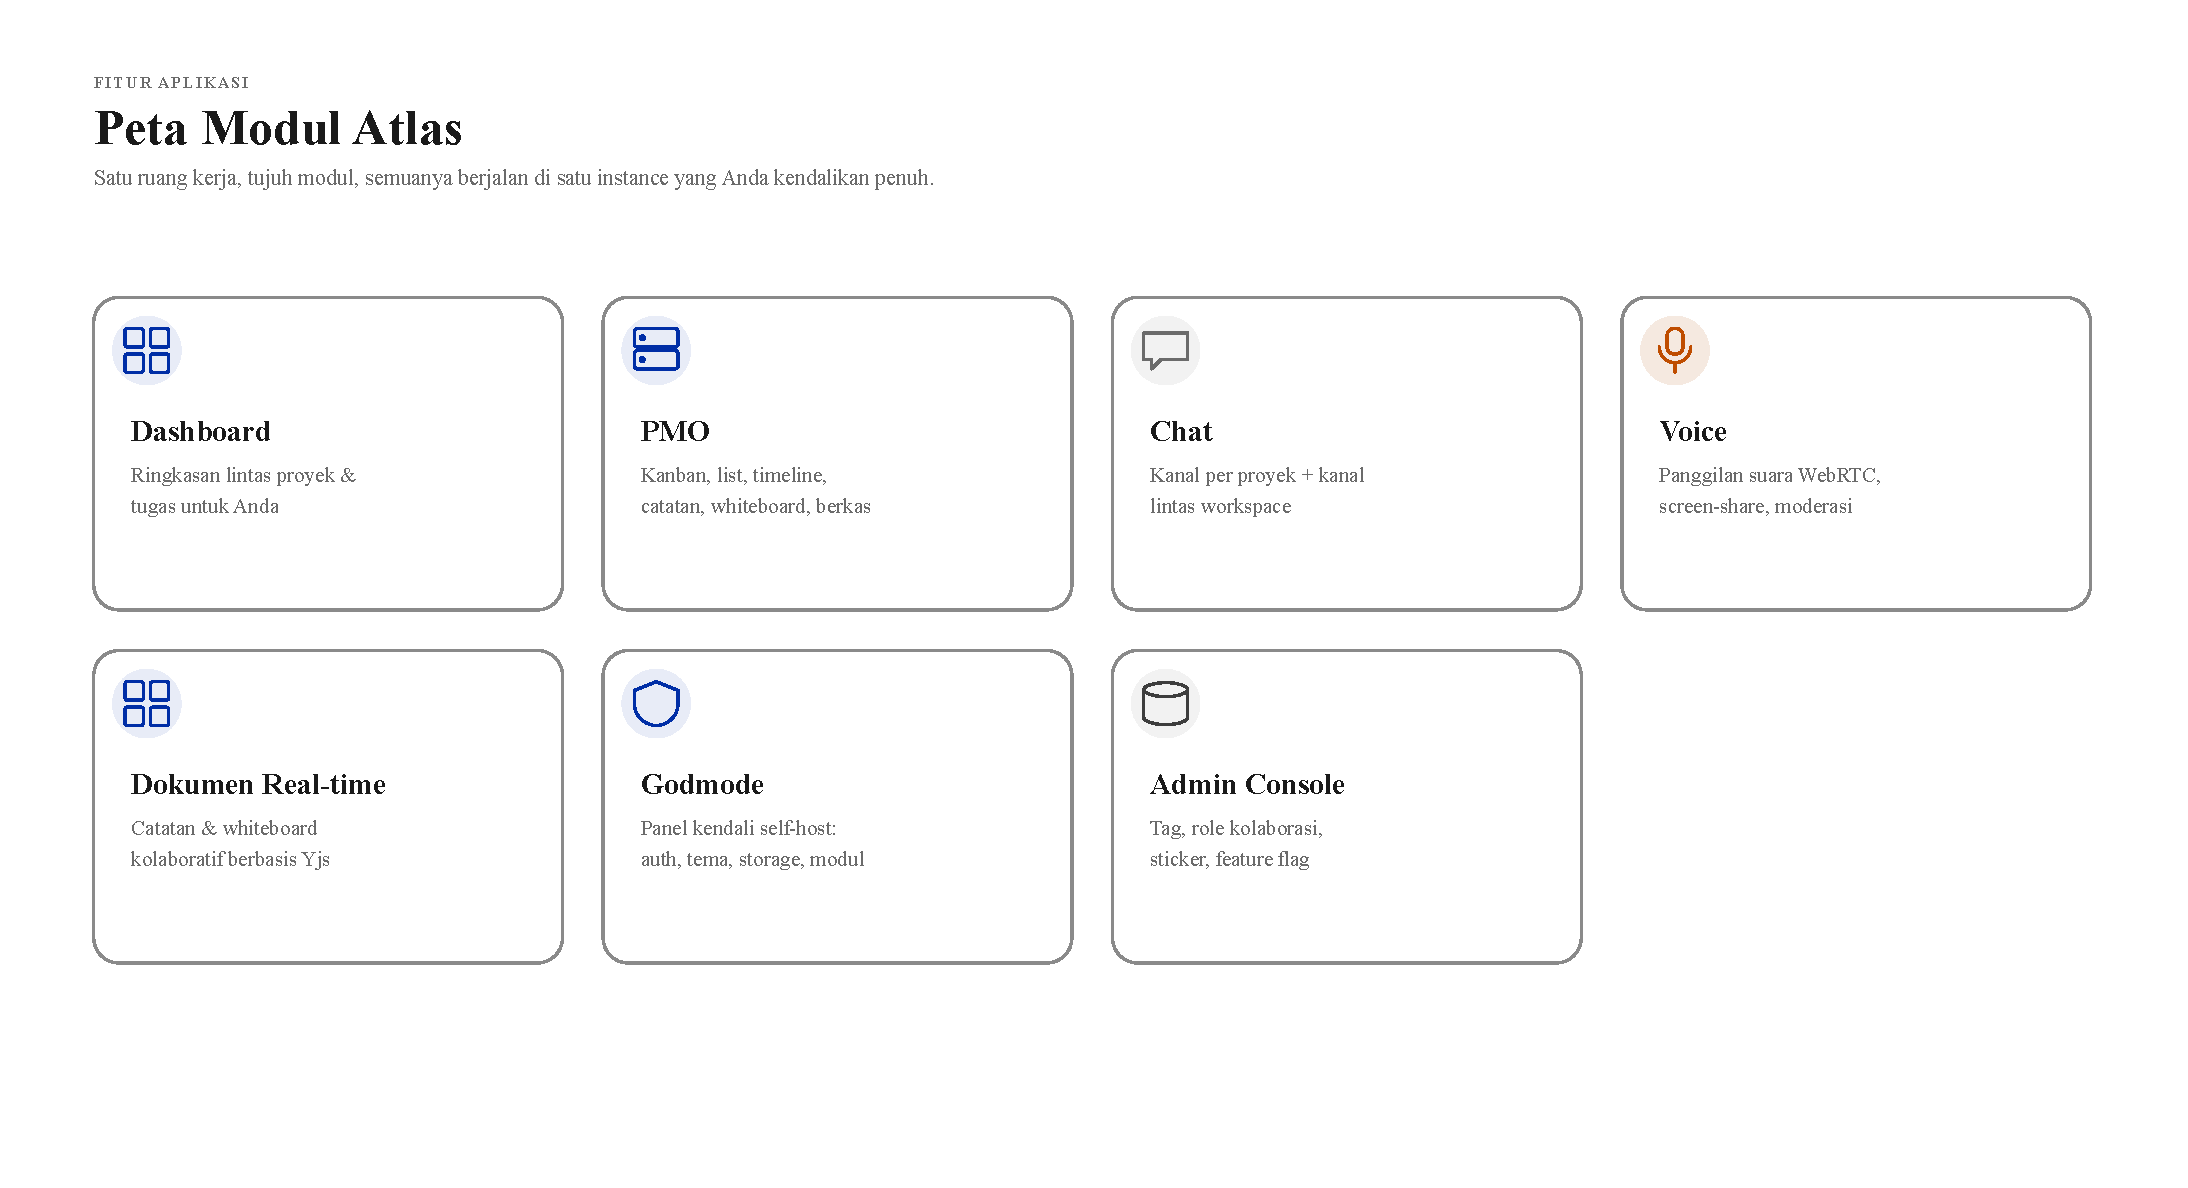
\includegraphics[width=0.72\linewidth]{assets/diagrams/feature-map.pdf}
\caption{Peta fitur Atlas. Setiap modul berbagi identitas pengguna, notifikasi, dan pencarian yang sama.}
\label{fig:feature-map}
\end{figure*}

\subsection{Manajemen Proyek (PMO)}

Setiap proyek memiliki daftar tugas yang bisa ditampilkan sebagai papan Kanban, tabel daftar, atau linimasa Gantt, lengkap dengan status, prioritas, penanggung jawab, dan tenggat waktu. Kunci penomoran tugas (mis.\ \texttt{NO10-14}) tetap unik dan berurutan per proyek meskipun tugas tersebar di banyak daftar berbeda (\cref{fig:pmo}).

\begin{figure*}[t]
\centering
\subfloat[Papan Kanban dengan kolom Backlog, In Progress, In Review, dan Done.]{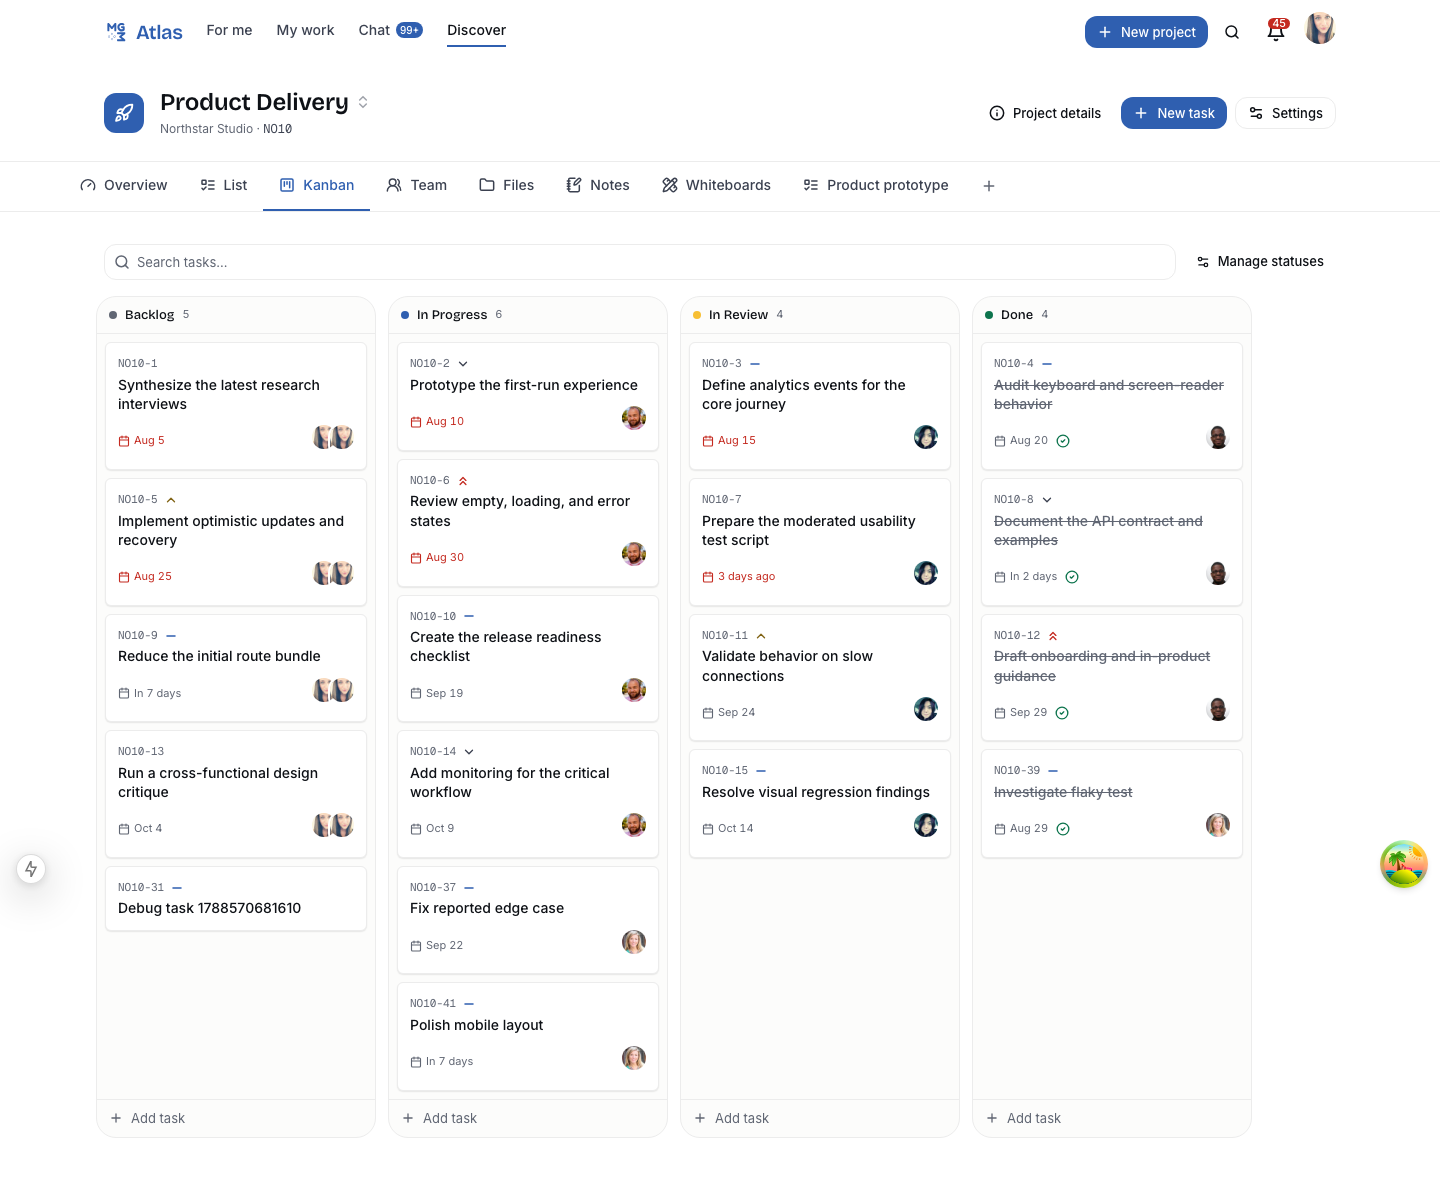
\includegraphics[width=0.485\linewidth]{assets/screenshots/curated/pmo-kanban.png}}\hfill
\subfloat[Detail tugas dibuka sebagai modal di atas papan, tanpa kehilangan konteks.]{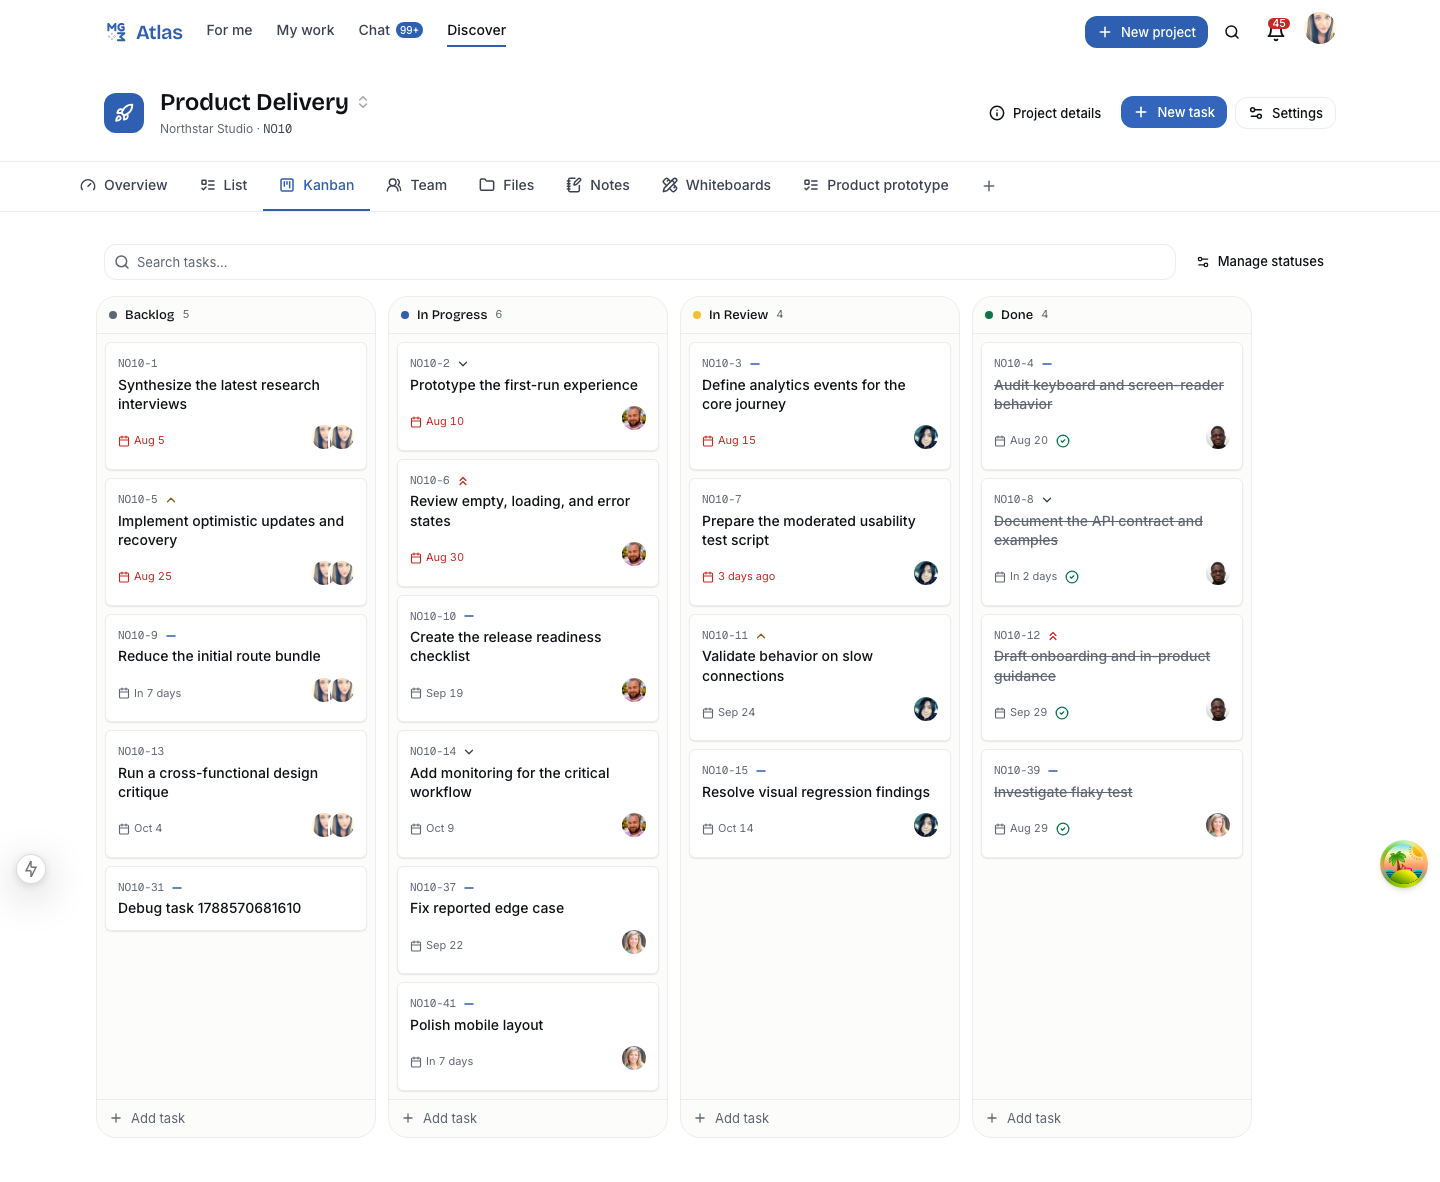
\includegraphics[width=0.485\linewidth]{assets/screenshots/curated/pmo-task-detail.png}}\\[4pt]
\subfloat[Linimasa Gantt untuk melihat jadwal seluruh tugas sekaligus.]{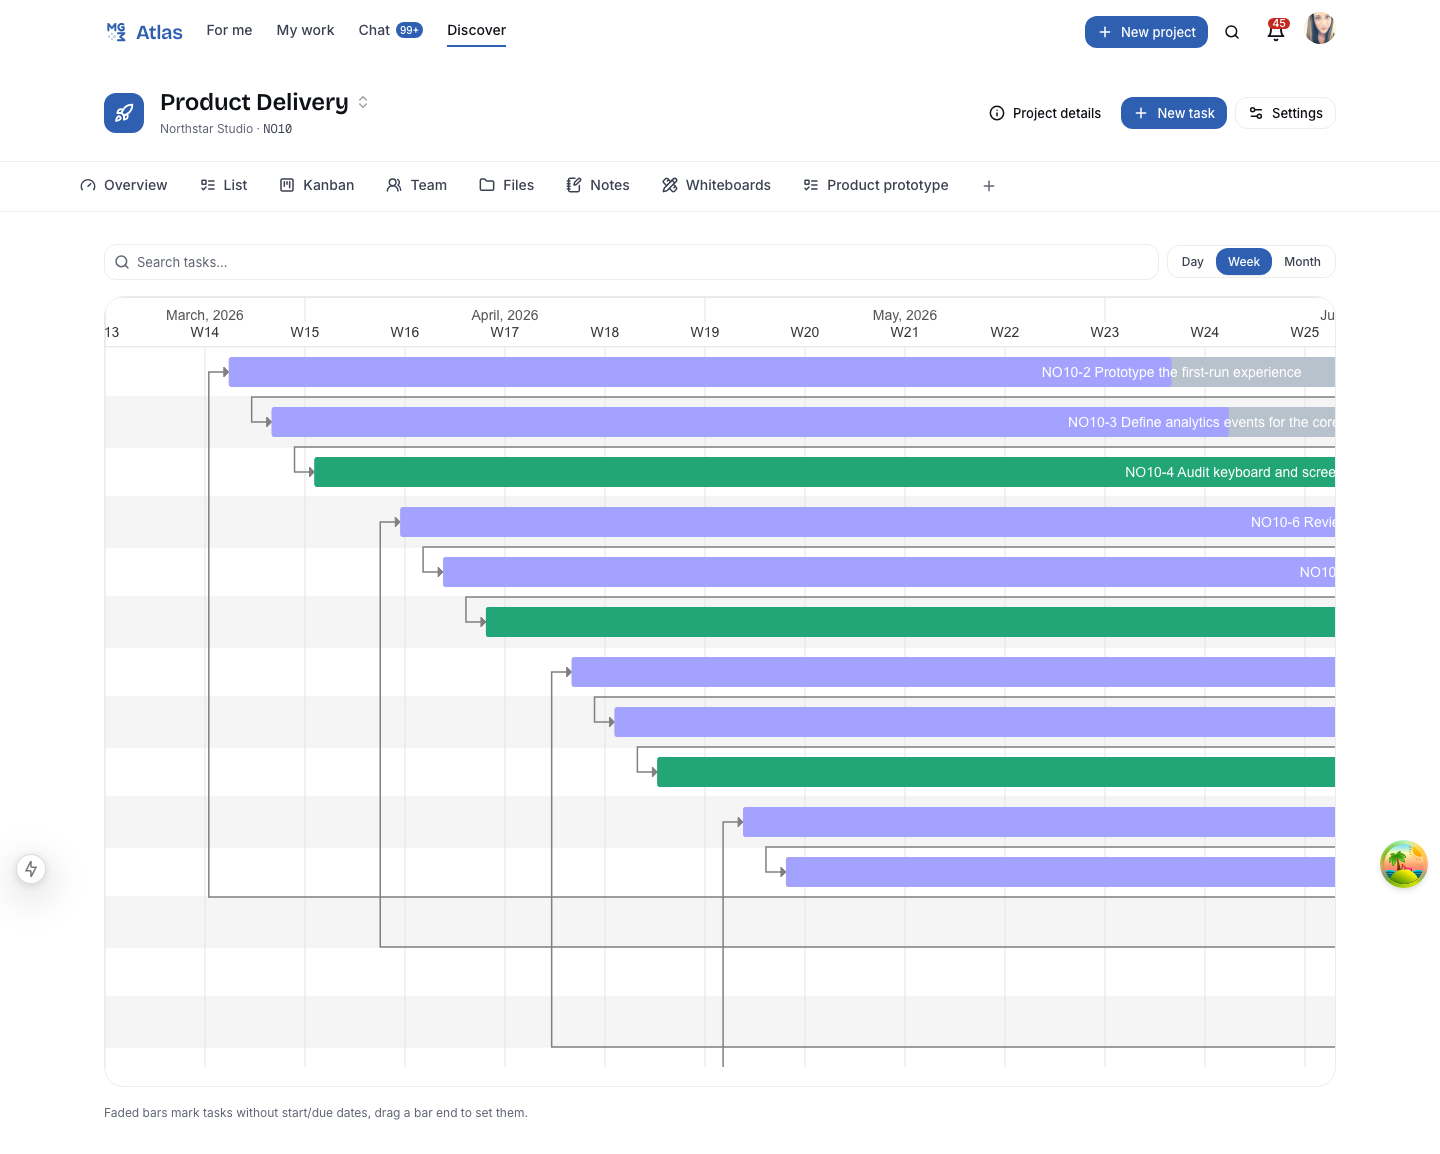
\includegraphics[width=0.485\linewidth]{assets/screenshots/curated/pmo-timeline.png}}\hfill
\subfloat[Whiteboard kolaboratif real-time (Yjs CRDT) untuk pemetaan ide.]{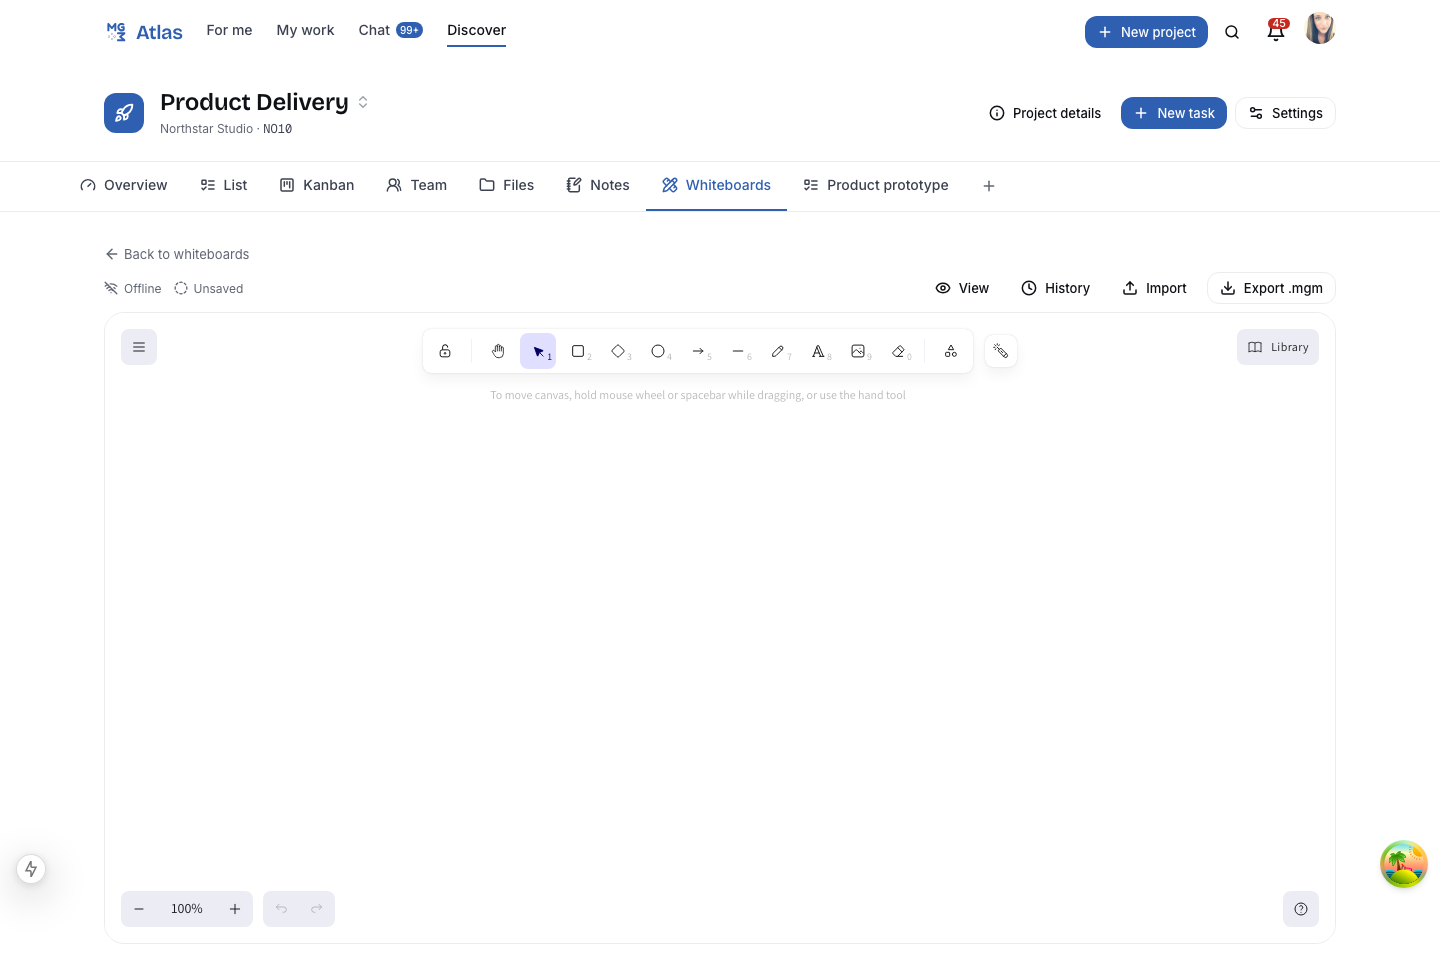
\includegraphics[width=0.485\linewidth]{assets/screenshots/curated/pmo-whiteboard.png}}
\caption{Empat tampilan modul PMO pada proyek yang sama.}
\label{fig:pmo}
\end{figure*}

\subsection{Obrolan Tim dan Panggilan Suara}

Setiap proyek memiliki kanal obrolannya sendiri, ditambah ruang obrolan lintas-tim (\textit{global}) untuk komunikasi seluruh organisasi. Pesan mendukung mention (\texttt{@nama}), reaksi emoji, stiker, lampiran berkas, dan pin. Panggilan suara berjalan lewat LiveKit (WebRTC), langsung antara peserta tanpa melewati server backend sebagai perantara media.

\begin{figure*}[t]
\centering
\subfloat[Obrolan proyek dengan mention, reaksi, dan lampiran.]{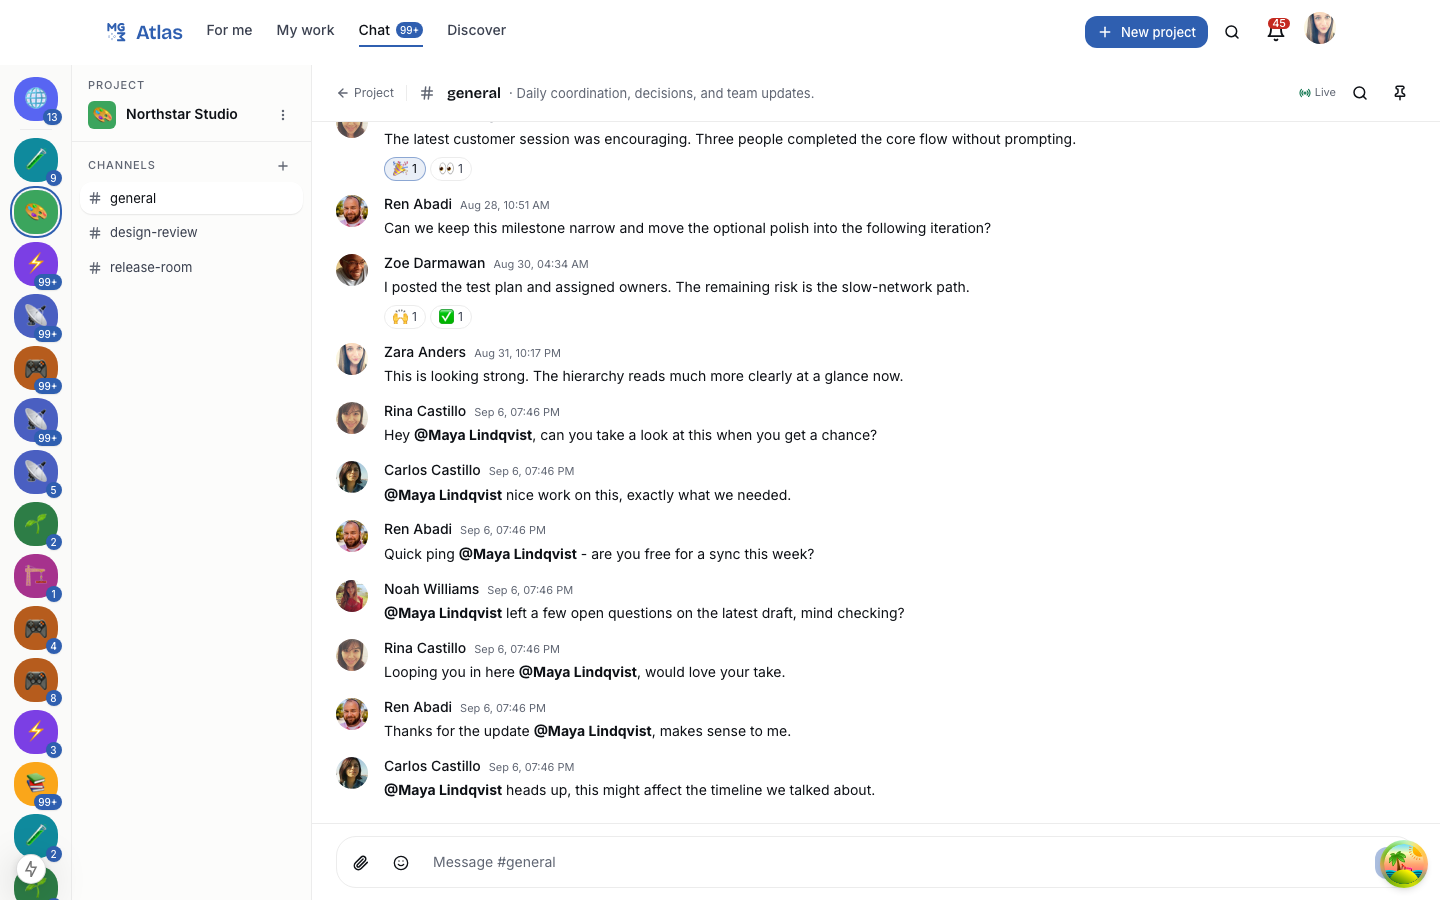
\includegraphics[width=0.485\linewidth]{assets/screenshots/curated/chat-project.png}}\hfill
\subfloat[Ruang suara real-time dengan kontrol mikrofon dan peserta aktif.]{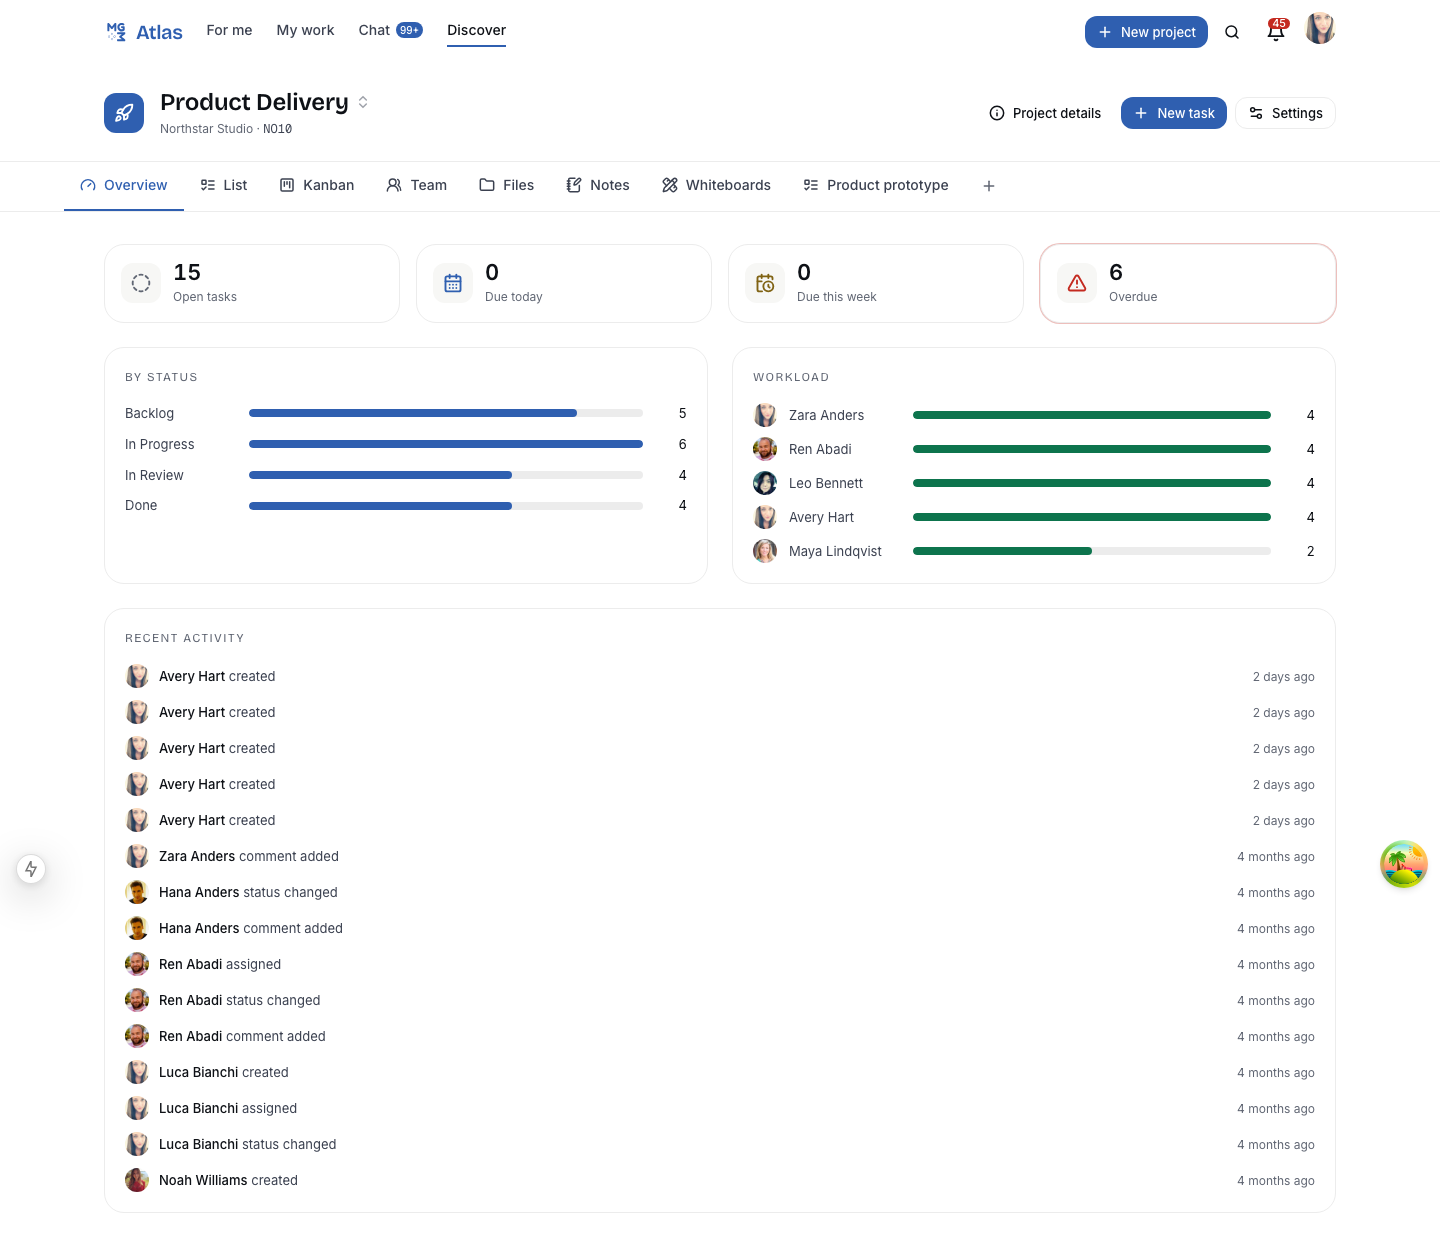
\includegraphics[width=0.485\linewidth]{assets/screenshots/curated/voice-room.png}}
\caption{Komunikasi tim: obrolan dan panggilan suara.}
\label{fig:chat-voice}
\end{figure*}

\subsection{Godmode: Panel Kendali Swa-hosting}

Godmode adalah panel superadmin yang membuat Atlas benar-benar layak dipakai organisasi lain tanpa bantuan developer: metode masuk, penyedia OAuth/SSO, penyimpanan berkas, tema tampilan, dan modul fitur, semuanya diatur lewat antarmuka, bukan berkas \texttt{.env}.

\begin{figure*}[t]
\centering
\subfloat[Ringkasan status instans dan progres konfigurasi awal.]{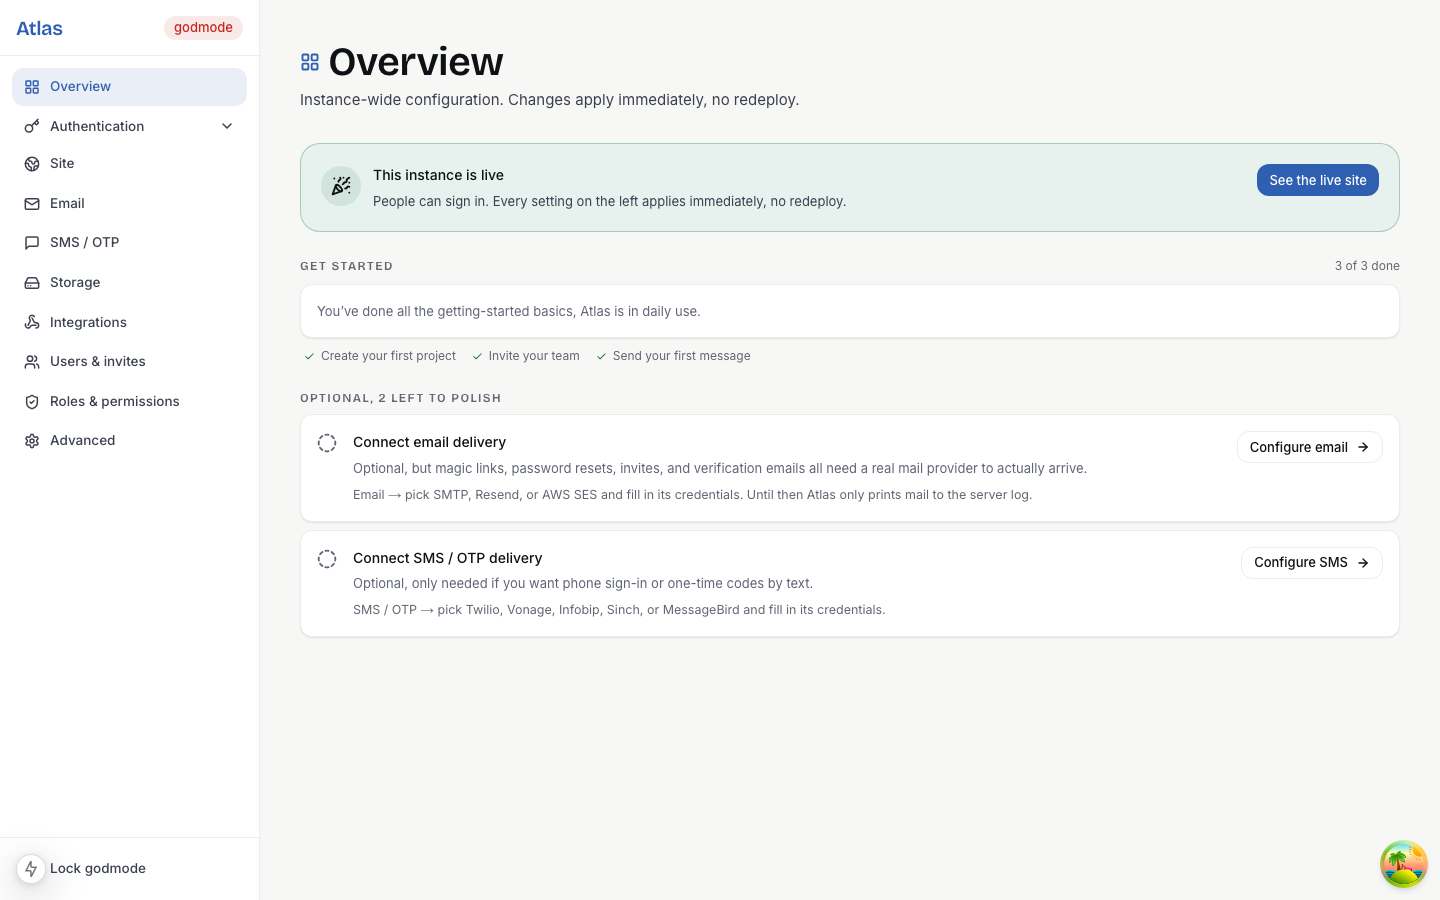
\includegraphics[width=0.485\linewidth]{assets/screenshots/curated/godmode-overview.png}}\hfill
\subfloat[Penyedia OAuth (Google, GitHub, Discord, dan lainnya) diaktifkan tanpa deploy ulang.]{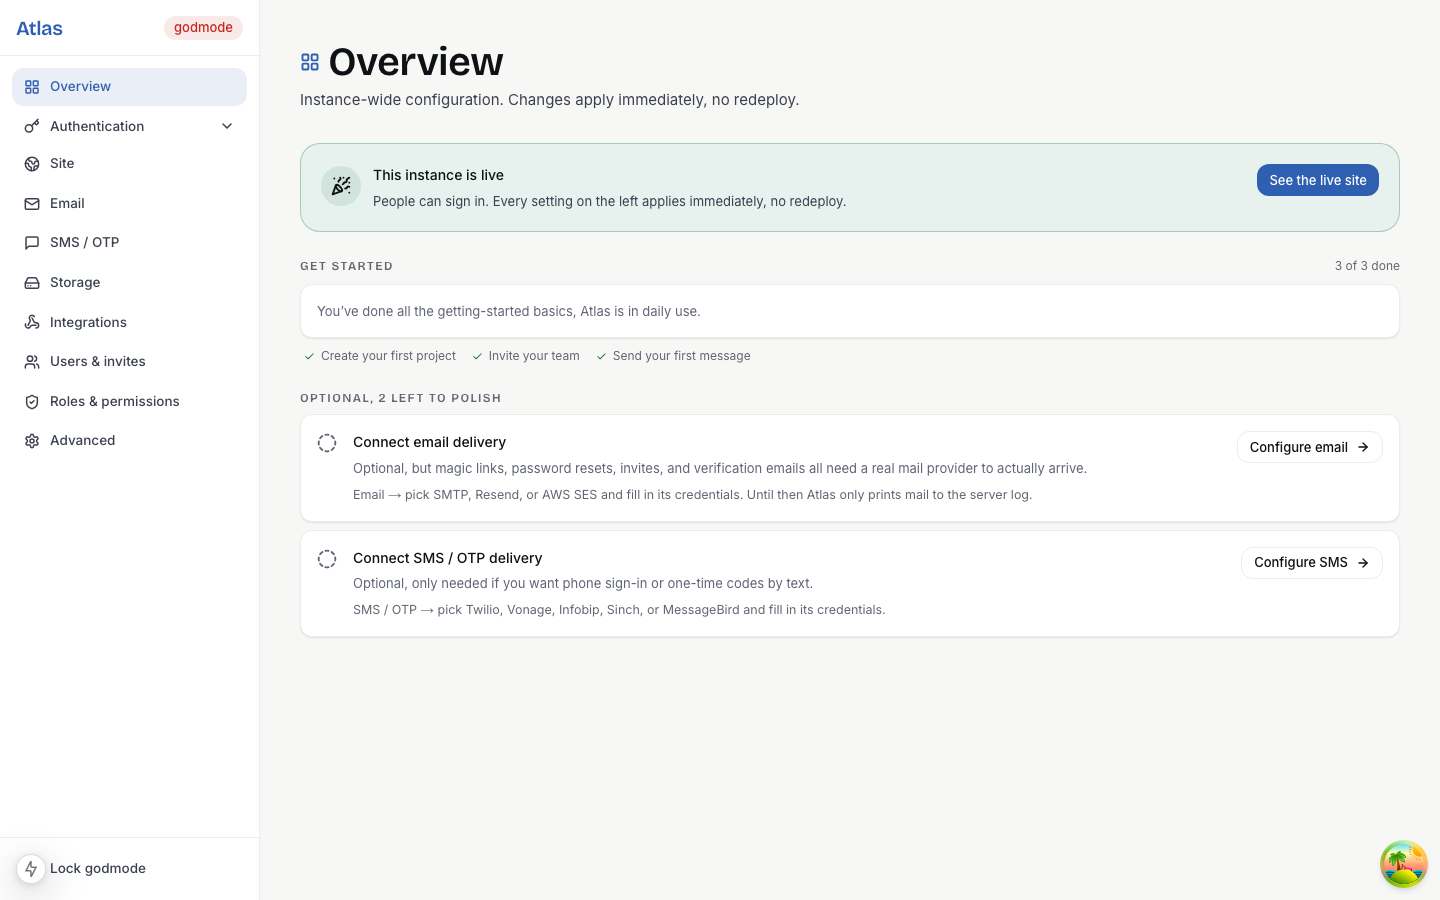
\includegraphics[width=0.485\linewidth]{assets/screenshots/curated/godmode-oauth.png}}
\caption{Godmode: ringkasan instans dan konfigurasi OAuth.}
\label{fig:godmode}
\end{figure*}

\subsection{24 Tema, Terang dan Gelap}

Setiap pengguna dapat memilih temanya sendiri dari 24 palet warna (masing-masing punya mode terang dan gelap), atau mengikuti tema bawaan yang ditetapkan admin. Seluruh tema melewati audit kontras WCAG otomatis sebelum bisa dirilis (\cref{fig:themes}).

\begin{figure*}[t]
\centering
\subfloat[Atlas Blue]{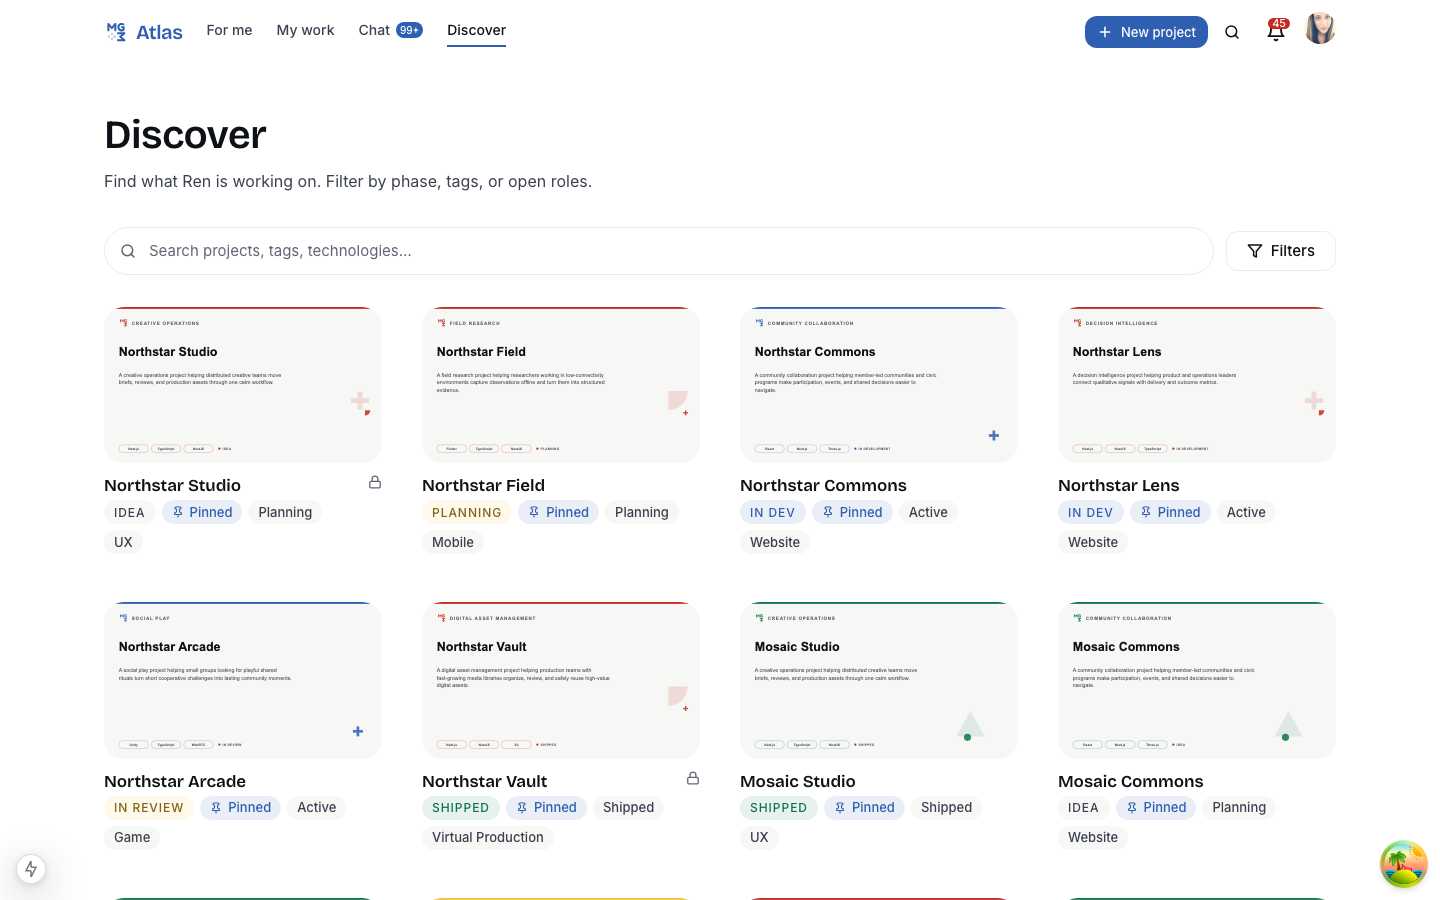
\includegraphics[width=0.24\linewidth]{assets/screenshots/curated/theme-atlas.png}}\hfill
\subfloat[Sunset]{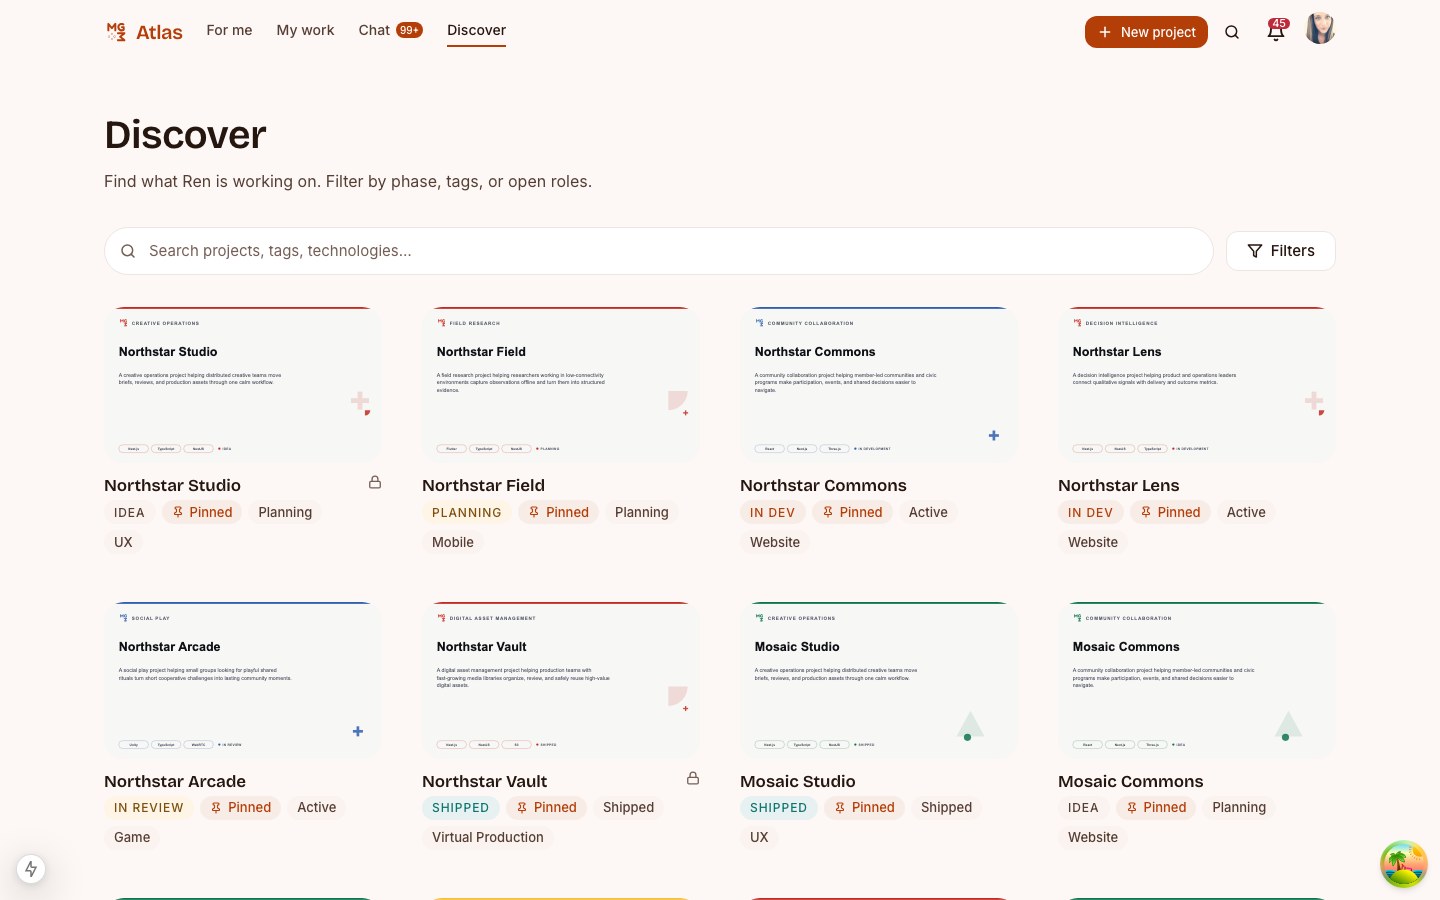
\includegraphics[width=0.24\linewidth]{assets/screenshots/curated/theme-sunset.png}}\hfill
\subfloat[Mint]{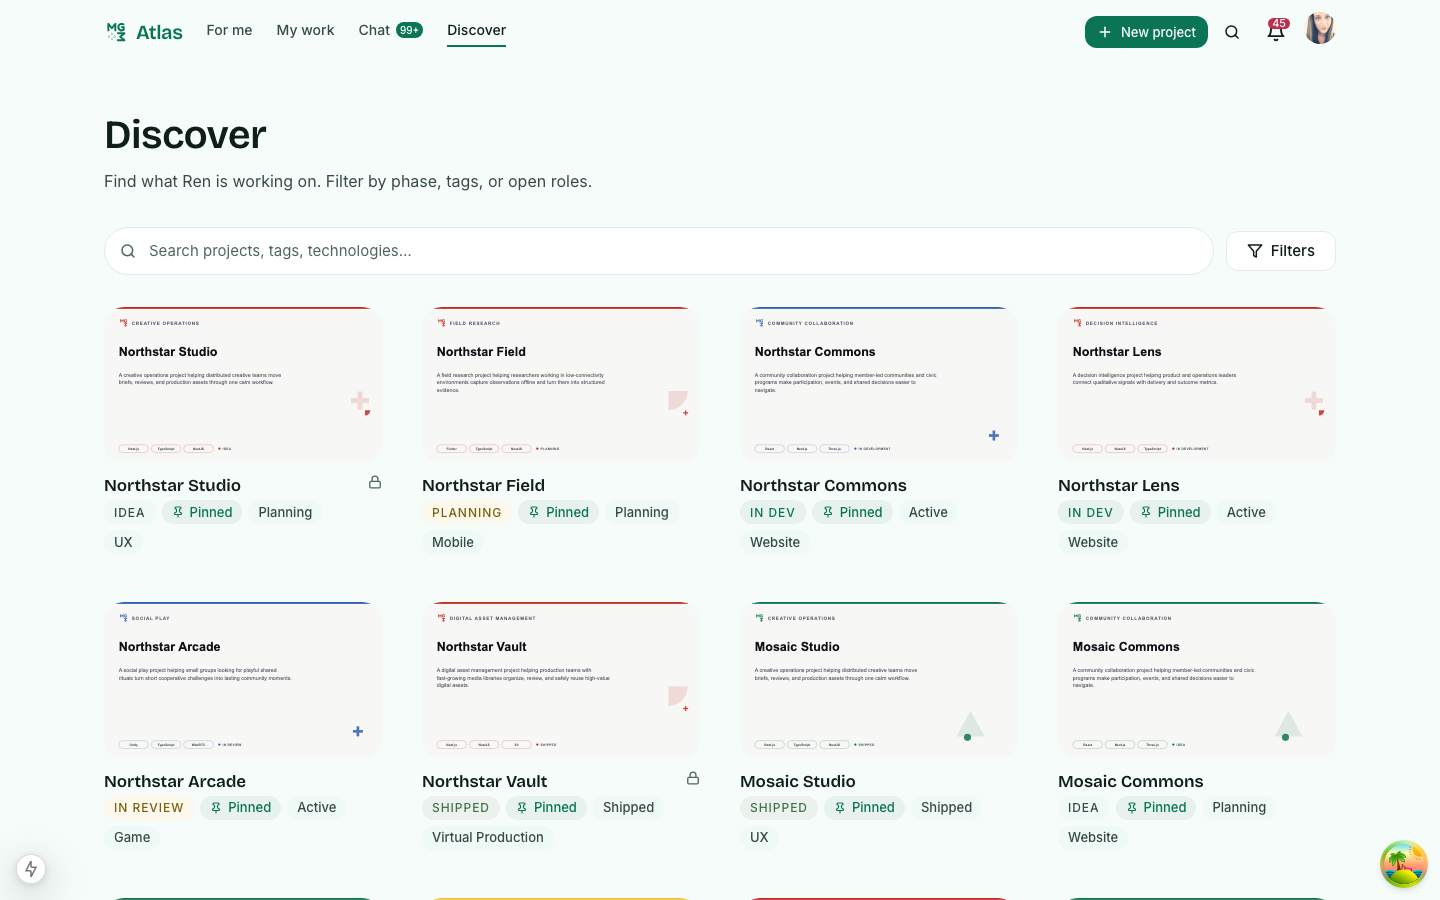
\includegraphics[width=0.24\linewidth]{assets/screenshots/curated/theme-mint.png}}\hfill
\subfloat[Lavender]{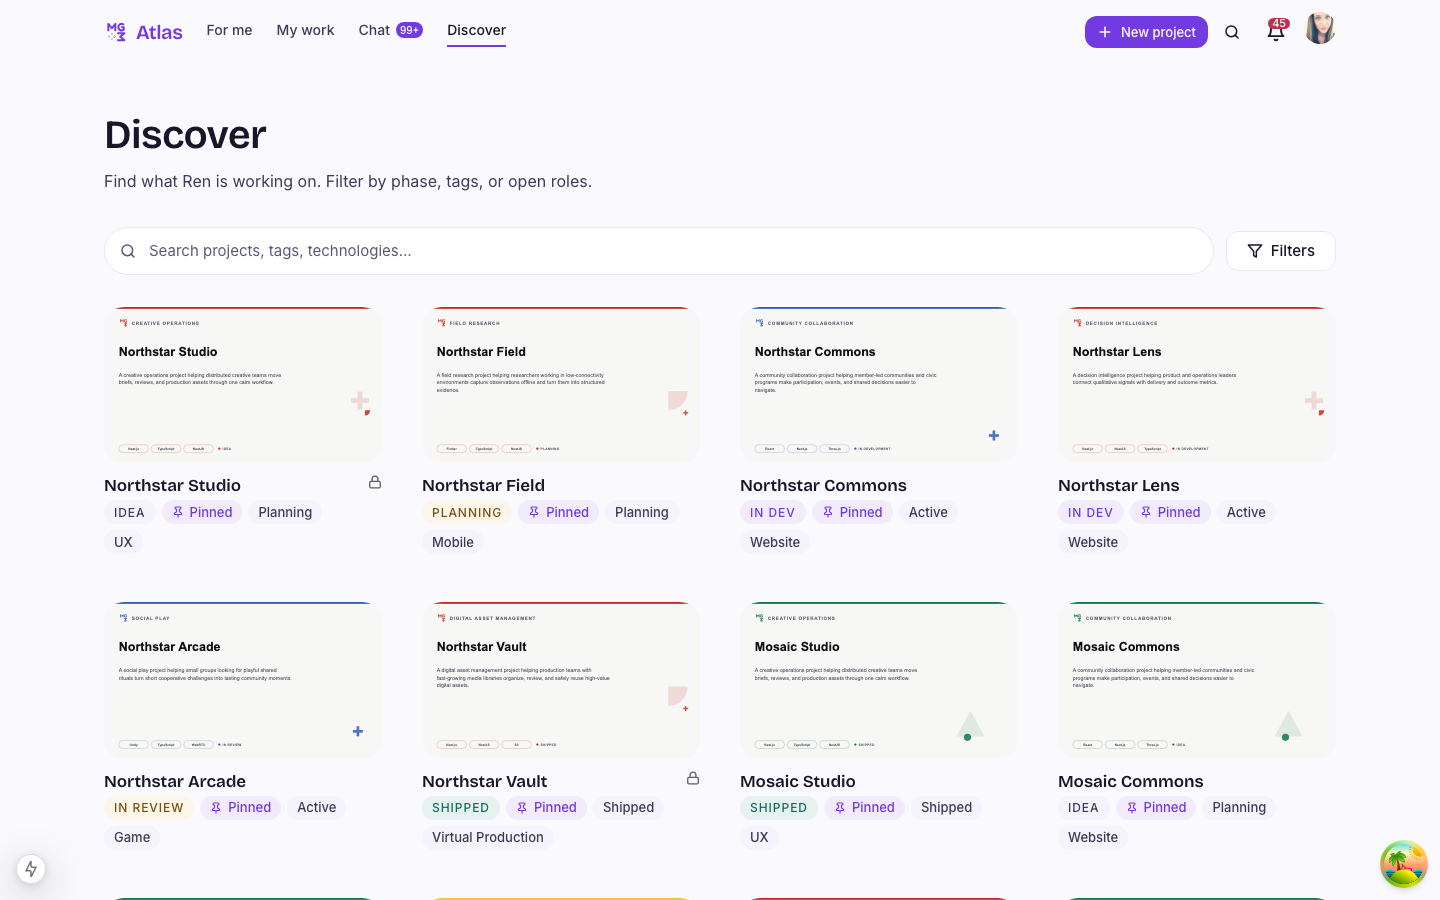
\includegraphics[width=0.24\linewidth]{assets/screenshots/curated/theme-lavender.png}}\\[4pt]
\subfloat[Deep Ocean]{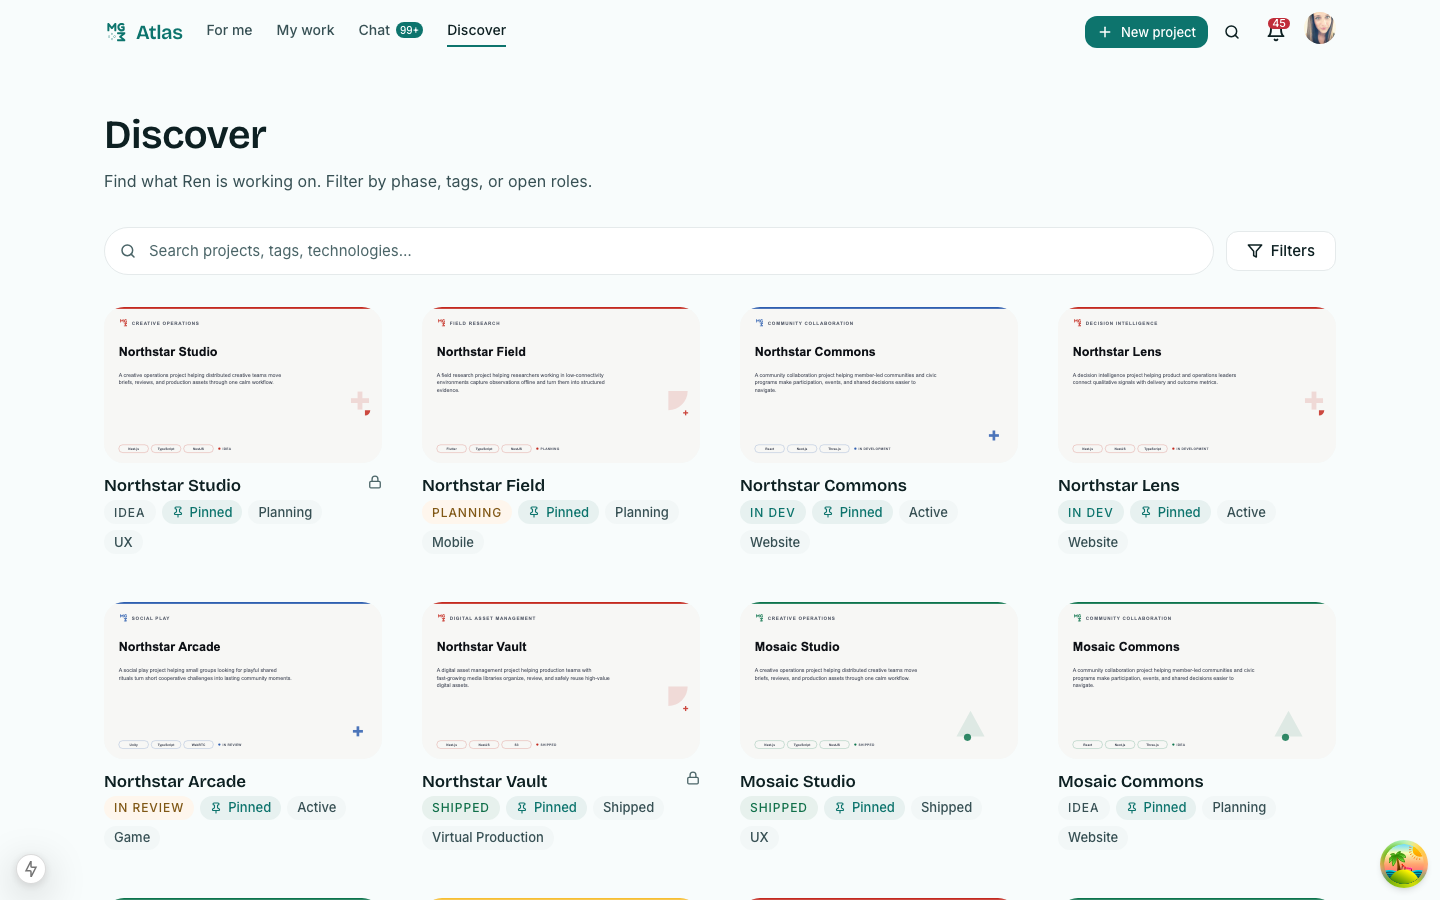
\includegraphics[width=0.24\linewidth]{assets/screenshots/curated/theme-ocean.png}}\hfill
\subfloat[Rose]{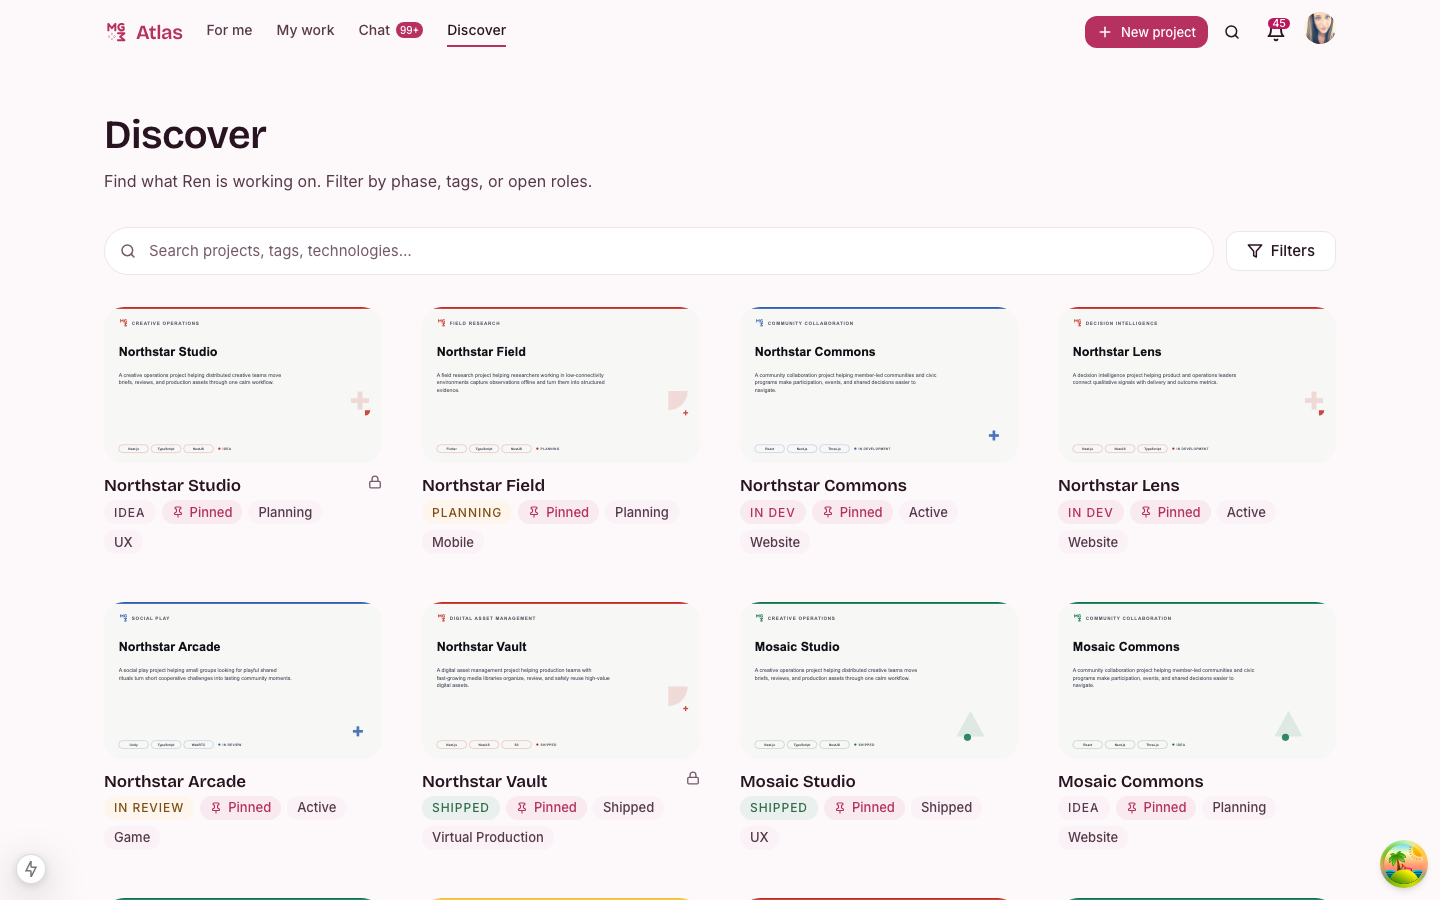
\includegraphics[width=0.24\linewidth]{assets/screenshots/curated/theme-rose.png}}\hfill
\subfloat[Midnight (gelap)]{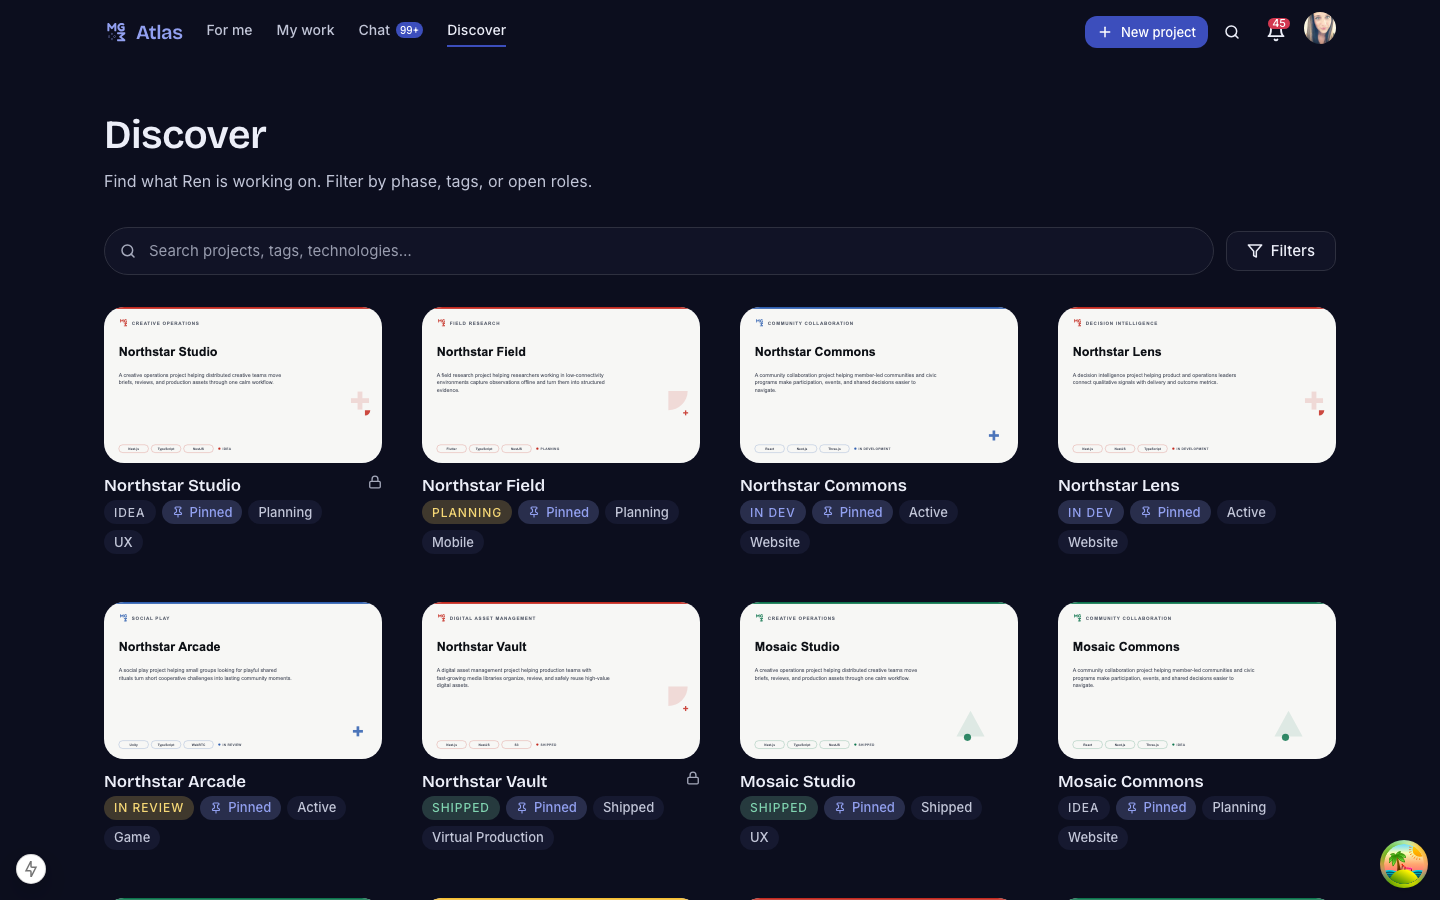
\includegraphics[width=0.24\linewidth]{assets/screenshots/curated/theme-midnight.png}}\hfill
\subfloat[Noir (gelap)]{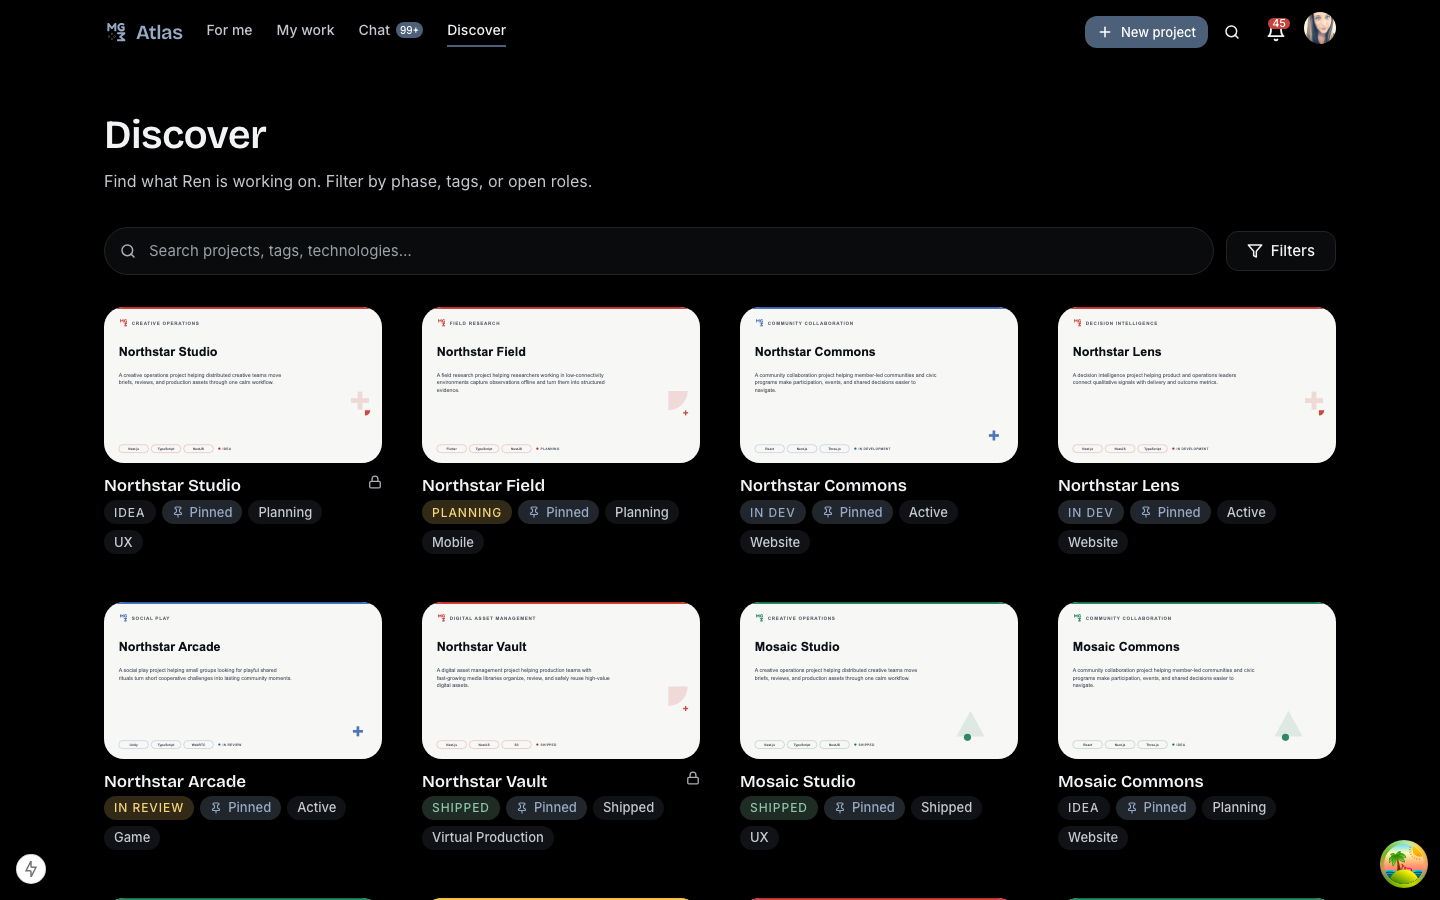
\includegraphics[width=0.24\linewidth]{assets/screenshots/curated/theme-noir.png}}
\caption{Delapan dari 24 tema yang tersedia, termasuk dua mode gelap.}
\label{fig:themes}
\end{figure*}

\subsection{Ringkasan modul lainnya}

\begin{description}
\item[Admin console.] Pengelolaan tag, peran kolaborasi, sticker, dan feature flag untuk operasional harian di luar Godmode.
\item[Catatan real-time.] Editor dokumen kolaboratif (BlockNote + Yjs) per daftar tugas, untuk brief, notulen, dan dokumentasi hidup.
\item[Notifikasi terpadu.] Satu pusat notifikasi untuk mention, penugasan tugas, dan pembaruan proyek, lintas seluruh modul.
\end{description}
